%
% main.tex -- Paper zum Thema <planet>
%
% (c) 2020 Autor, OST Ostschweizer Fachhochschule
%
% !TEX root = ../../buch.tex
% !TEX encoding = UTF-8
%
\chapter{Warum sind Planeten Sphären?\label{chapter:planet}}
\kopflinks{Warum sind Planeten Sphären?}
\begin{refsection}
\chapterauthor{Jakob Gierer und Lukas Schöpf}

Ein paar Hinweise für die korrekte Formatierung des Textes
\begin{itemize}
\item
Absätze werden gebildet, indem man eine Leerzeile einfügt.
Die Verwendung von \verb+\\+ ist nur in Tabellen und Arrays gestattet.
\item
Die explizite Platzierung von Bildern ist nicht erlaubt, entsprechende
Optionen werden gelöscht. 
Verwenden Sie Labels und Verweise, um auf Bilder hinzuweisen.
\item
Beginnen Sie jeden Satz auf einer neuen Zeile. 
Damit ermöglichen Sie dem Versionsverwaltungssysteme, Änderungen
in verschiedenen Sätzen von verschiedenen Autoren ohne Konflikt 
anzuwenden.
\item 
Bilden Sie auch für Formeln kurze Zeilen, einerseits der besseren
Übersicht wegen, aber auch um GIT die Arbeit zu erleichtern.
\end{itemize}

%
% einleitung.tex -- Beispiel-File für die Einleitung
%
% (c) 2020 Prof Dr Andreas Müller, Hochschule Rapperswil
%
% !TEX root = ../../buch.tex
% !TEX encoding = UTF-8
%
\section{Einleitung\label{planet:section:einleitung}}
\rhead{Einleitung}
Was ist eigentlich ein Planet?
Wie Unterscheidet man einen Planet von einem Zwergplanet?
Genau diese Fragen stellten sich Wissenschaftler im Jahr 2006 \cite{planet:iaub5}.
Die Definition auf welche sich geeinigt wurde sieht folgendermassen aus.
Ein Planet ist ein Himmelskörper welcher:
\begin{itemize}
	\item einen Orbit um eine Sonne hat,
	\item hat ausreichende Masse, damit seine Eigengravitation die Kräfte eines starren Körpers überwinden kann, sodass es eine hydrostatische Gleichgewichtsform (nahezu rund) annimmt, und
	\item hat die Umgebung seiner Umlaufbahn freigeräumt.
\end{itemize}

In diesem Kapitel wird sich mit der hydrostatische Gleichgewichtsform befasst.
Sie wird in 2D und in 3D hergeleitet



%
% teil1.tex -- Beispiel-File für das Paper
%
% (c) 2020 Prof Dr Andreas Müller, Hochschule Rapperswil
%
% !TEX root = ../../buch.tex
% !TEX encoding = UTF-8
%
\section{Teil 1
\label{beispiel:section:teil1}}
\rhead{Problemstellung}
Sed ut perspiciatis unde omnis iste natus error sit voluptatem
accusantium doloremque laudantium, totam rem aperiam, eaque ipsa
quae ab illo inventore veritatis et quasi architecto beatae vitae
dicta sunt explicabo.
Nemo enim ipsam voluptatem quia voluptas sit aspernatur aut odit
aut fugit, sed quia consequuntur magni dolores eos qui ratione
voluptatem sequi nesciunt
\begin{equation}
\int_a^b x^2\, dx
=
\left[ \frac13 x^3 \right]_a^b
=
\frac{b^3-a^3}3.
\label{beispiel:equation1}
\end{equation}
Neque porro quisquam est, qui dolorem ipsum quia dolor sit amet,
consectetur, adipisci velit, sed quia non numquam eius modi tempora
incidunt ut labore et dolore magnam aliquam quaerat voluptatem.

Ut enim ad minima veniam, quis nostrum exercitationem ullam corporis
suscipit laboriosam, nisi ut aliquid ex ea commodi consequatur?
Quis autem vel eum iure reprehenderit qui in ea voluptate velit
esse quam nihil molestiae consequatur, vel illum qui dolorem eum
fugiat quo voluptas nulla pariatur?

\subsection{De finibus bonorum et malorum
\label{beispiel:subsection:finibus}}
At vero eos et accusamus et iusto odio dignissimos ducimus qui
blanditiis praesentium voluptatum deleniti atque corrupti quos
dolores et quas molestias excepturi sint occaecati cupiditate non
provident, similique sunt in culpa qui officia deserunt mollitia
animi, id est laborum et dolorum fuga \eqref{beispiel:equation1}.

Et harum quidem rerum facilis est et expedita distinctio
\ref{beispiel:section:teil2}.
Nam libero tempore, cum soluta nobis est eligendi optio cumque nihil
impedit quo minus id quod maxime placeat facere possimus, omnis
voluptas assumenda est, omnis dolor repellendus
\ref{beispiel:section:teil3}.
Temporibus autem quibusdam et aut officiis debitis aut rerum
necessitatibus saepe eveniet ut et voluptates repudiandae sint et
molestiae non recusandae.
Itaque earum rerum hic tenetur a sapiente delectus, ut aut reiciendis
voluptatibus maiores alias consequatur aut perferendis doloribus
asperiores repellat.



%
% 2_Multipol.tex
%
% (c) 2020 Prof Dr Andreas Müller, Hochschule Rapperswil
%
% !TEX root = ../../buch.tex
% !TEX encoding = UTF-8
%
\section{Multipolmoment
\label{planet:section:multipol}}
\rhead{Multipolmoment}
In der Physik ist die Multipolentwicklung ein Verfaheren, um die Poisson-Gleichung im dreidimensionalen Raum zu lösen, bei der eine Laurent-Reihe als Lösungsfunktion entsteht.
Die Entwicklungskoeffizienten dieser Reihe heissen Multipolmomente.
Diese Methode wird hauptsächlich in der Elektrostatik und Magnetostatik verwendet, kann aber auf jedem Gebiet der Physik verallgemeinert werden, in dem die Poisson-Gleichung auftritt.

Die Motivation der Multipolentwicklung liegt darin, das Verhalten von beliebigen Potentialen (Gravitationspotential) in grosser Entfernung zu betrachten.
Analog zur Fourier-Theorie lässt sich mit der Multipolentwicklung ein komplexe physikalisches Problem in kleinere Teilprobleme aufteilen die leichter zu lösen sind.
Die \cref{planet:fig:multipol} zeigt die ersten Entwicklungsschritte einer Ladungswolke.
Desweiteren zeigt sich auch, dass die Bewegungsgleichung für Planeten im wesentlichen zu linearen Differentialgleichungen für die Multipolkoeffizienten werden.
Alle Koeffizienten konvergieren gegen 0, ausser dem konstanten Koeffizienten, dieser ergibt die Kugelform.

Dieser Abschnitt und die Herleitungen basieren auf den Inhalten von \cite{planet:multi} und \cite{planet:quadro}.

\begin{figure}[h!]
    \centering
    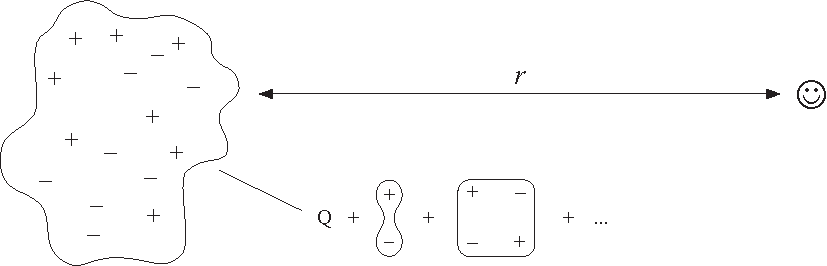
\includegraphics[width=\linewidth]{papers/planet/pictures/Multipol.pdf}
    \caption{Darstellung der Multipolentwicklung
        \label{planet:fig:multipol}}
\end{figure}

\subsection{Grundlagen
\label{planet:subsection:grundlagen}}

Die Poisson-Gleichung lässt sich allgemein als

\begin{equation*}
\Delta \phi (\vec{r}) = - f (\vec{r})
\end{equation*}

\noindent
schreiben, wobei \(\Delta\) der Laplace-Operator, \(f\) eine Dichte und \(\phi\) ein Potential ist (das Minus ist Konvention).
Die formale Lösung dieser Gleichung ist

\begin{equation*}
\phi (\vec{r}) = \frac{1}{4\pi} \int d^3 \vec{r}\,' \frac{f (\vec{r}\,')} {\abs{\vec{r} - \vec{r}\,'}}.
\end{equation*}

\noindent
Ist \(f (\vec{r})\) in einem Volumen lokalisiert, kann für Orte \(\vec{r}\), die weit ausserhalb dieses Volumens liegen, \(r \gg r\,'\), der Bruch in eine Taylor-Reihe in \(\vec{r}\,'\) um \(\vec{r}\,' = 0\) entwickelt werden:

\begin{equation*}
\frac{1}{\abs{\vec{r} - \vec{r}\,'}} = \sum_{n=0}^{\infty} \frac{1}{n!} \left( \vec{r}\,' \cdot \vec{\nabla}\,' \right)^n \left. \frac{1}{\abs{\vec{r} - \vec{r}\,'}} \right|_{\vec{r}\,'=0}
\end{equation*}

\noindent
Dabei bedeutet \(\vec{\nabla}\,'\), dass der Nablaoperator \(\vec{\nabla}\) nur auf die gestrichenen Koordinaten \(\vec{r}\,'\) und nicht auf \(\vec{r}\) wirkt.
Nach Bilden der Ableitungen wird diese an der Stelle \(\vec{r}\,' = 0\) ausgewertet.
Durch Umformen erhält man

\begin{equation*}
\frac{1}{\abs{ \vec{r} - \vec{r}\,'}} = \sum_{n=0}^{\infty} \frac{1}{n!} \left( - \vec{r}\,' \cdot \vec{\nabla} \right)^n \frac{1}{r}.
\end{equation*}

\noindent
Die genaue Form der Entwicklung und der Multipole hängt vom jeweiligen Koordinatensystem ab.

\subsection{Kartesische Multpolentwicklung
\label{planet:subsection:kartentwicklung}}

Die kartesische Multipolentwicklung wird im kartesischen Koordinatensystem durchgeführt.
Dort ist

\begin{equation*}
\vec{r}\,' \cdot \vec{\nabla} = r\,'_{i} \partial_{i},
\end{equation*}

\noindent
wobei die Einsteinsche Summenkonvention verwendet wird.
Dann muss bei einem Summanden \(n\)-ter Ordnung ein Tensor \(n\)-ter Stufe, nämlich \(\textstyle \prod_{k=1}^{n} \partial_{i_{k}} \frac{1}{r}\) berechnet werden:


\begin{align*}
\frac{1}{\abs{ \vec{r} - \vec{r}\,'}} &= \frac{1}{r} - r\,'_{i} \partial_{i} \frac{1}{r} + \frac{1}{2} r\,'_{i} r\,'_{j} \partial_{i} \partial_{j} \frac{1}{r} + \mathcal{O}(r\,'^{3}) \\
&= \frac{1}{r} + r\,'_{i} \frac{r_{i}}{r^{3}} + \frac{1}{2} r\,'_{i} r\,'_{j} \frac{3 r_{i} r_{j} - r^{2} \delta_{ij}}{r^{5}} + \mathcal{O}(r\,'^{3}).
\end{align*}


\noindent
Das Symbol \(\delta_{i\!j}\) repräsentiert das sogenannte Kronecker-Delta.
Die formale Lösung \(\phi (\vec{r})\) der Poisson-Gleichung ist unter Verwendung der Identität \(r\,'_{i} r\,'_{j} r^{2} \delta_{i\!j} = r\,'^{2} r_{i} r_{j} \delta_{i\!j}\) wie folgt darstellbar:


\begin{align*}
\phi (\vec{r}) &= \frac{1}{4\pi} \left[ \frac{1}{r} \underbrace{\int f (\vec{r}\,') \, d^3 \vec{r}\,'}_{\text{Monopol-}} + \frac{r_{i}}{r^{3}} \underbrace{\int d^3 \vec{r}\,' \, r\,'_{i} f (\vec{r}\,')}_{\text{Dipol-}} + \frac{1}{2} \frac{r_{i} r_{j}}{r^{5}} \underbrace{\int d^3 \vec{r}\,' \left( 3 r\,'_{i} r\,'_{j} - r\,'^{2} \delta_{i\!j} \right) f (\vec{r}\,')}_{\text{Quadrupolmoment}} \dots \right] \\
&= \frac{1}{4\pi} \left[ \frac{1}{r} q + \frac{r_{i}}{r^{3}} p_{i} + \frac{1}{2} \frac{r_{i} r_{j}}{r^{5}} Q_{i\!j} + \dots \right].
\end{align*}


In der entwickelten Reihe kommen die Faktoren \(r\) im Nenner mit steigendem Exponenten vor.
Dabei werden die höheren Ordnungen der Multipolmomente, mit zuhnemendem Abstand zum beobachteten Volumen immer weiter vernachlässigbar.
Es wurde einfachheitshalber für die Berechnungen der Kugelform in diesem Kapitel als Approximation das erste Moment verwendet und die höheren vernachlässigt.



\subsection{Anwendung
\label{planet:subsection:anwendung}}

Die Gravitation hat im Gegensatz zum Elektromagnetismus nur positive Ladungen, die Massen.
Es können dennoch gravitative Multipole definiert werden.
Aus der Poisson-Gleichung des Newtonschen Gravitationsgesetzes

\begin{equation*}
    \Delta \phi = -4\pi G\rho
\end{equation*}

\noindent
mit der Gravitationskonstante \(G\) und der Massendichte \(\rho\) ist der gravitative Monopol die Gesamtmasse \(M\).

Da Massen nur positiv sind, lässt sich aus den Ladungen kein Dipolmoment bilden.
Aus diesem Grund ist der gravitative Quadrupol nicht über zwei Dipole definiert.
Dennoch haben Massenverteilungen Quadrupole.
\cref{planet:fig:quadroearth} zeigt ein solches wobei, die blau gefärbten Abweichungen, das fehlen der Masse als negative Masse gesehen wird und die rot gefärbten Abweichungen, die überschüssigen Massen als positive Massen betrachtet wird.  

\begin{figure}[h]
    \centering
    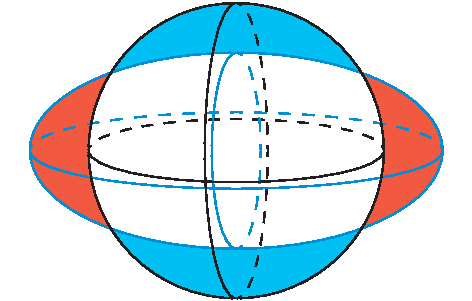
\includegraphics[width=0.60\linewidth]{papers/planet/pictures/Quadroearth.pdf}
    \caption{Beispiel eines gravitativen Quadrupol
        \label{planet:fig:quadroearth}}
\end{figure}

\begin{beispiel}
    Die Erde ist durch ihre Rotation keine perfekte Kugel, sie ist leicht eingedellt an den Polen und am Äquator bildet sich ein Wulst (\cref{planet:fig:quadroearth}).
    Die Schwerkraft versucht den höhren Multipolen entgegenzuwirken.
    Desweiteren sind durch bestimmte Dichteunterschiede weitere Abweichungen der Kugelform, in \cref{planet:fig:geoid} ersichtlich.
\end{beispiel}

Einige himmelsmechanische Phänomene, wie die dynamische Entwicklung der Bahnelemente von Satelliten, lassen sich mit dem daraus resultierenden Quadrupolmoment beschreiben.

%
% teil3.tex -- Beispiel-File für Teil 3
%
% (c) 2020 Prof Dr Andreas Müller, Hochschule Rapperswil
%
% !TEX root = ../../buch.tex
% !TEX encoding = UTF-8
%
\section{Teil 3
\label{000template:section:teil3}}
\rhead{Teil 3}
Sed ut perspiciatis unde omnis iste natus error sit voluptatem
accusantium doloremque laudantium, totam rem aperiam, eaque ipsa
quae ab illo inventore veritatis et quasi architecto beatae vitae
dicta sunt explicabo. Nemo enim ipsam voluptatem quia voluptas sit
aspernatur aut odit aut fugit, sed quia consequuntur magni dolores
eos qui ratione voluptatem sequi nesciunt. Neque porro quisquam
est, qui dolorem ipsum quia dolor sit amet, consectetur, adipisci
velit, sed quia non numquam eius modi tempora incidunt ut labore
et dolore magnam aliquam quaerat voluptatem. Ut enim ad minima
veniam, quis nostrum exercitationem ullam corporis suscipit laboriosam,
nisi ut aliquid ex ea commodi consequatur? Quis autem vel eum iure
reprehenderit qui in ea voluptate velit esse quam nihil molestiae
consequatur, vel illum qui dolorem eum fugiat quo voluptas nulla
pariatur?

\subsection{De finibus bonorum et malorum
\label{000template:subsection:malorum}}
At vero eos et accusamus et iusto odio dignissimos ducimus qui
blanditiis praesentium voluptatum deleniti atque corrupti quos
dolores et quas molestias excepturi sint occaecati cupiditate non
provident, similique sunt in culpa qui officia deserunt mollitia
animi, id est laborum et dolorum fuga. Et harum quidem rerum facilis
est et expedita distinctio. Nam libero tempore, cum soluta nobis
est eligendi optio cumque nihil impedit quo minus id quod maxime
placeat facere possimus, omnis voluptas assumenda est, omnis dolor
repellendus. Temporibus autem quibusdam et aut officiis debitis aut
rerum necessitatibus saepe eveniet ut et voluptates repudiandae
sint et molestiae non recusandae. Itaque earum rerum hic tenetur a
sapiente delectus, ut aut reiciendis voluptatibus maiores alias
consequatur aut perferendis doloribus asperiores repellat.




\printbibliography[heading=subbibliography]
\end{refsection}
